% Dokumentklasse --------------
\documentclass[12pt,naustrian,a4widepaper]{scrartcl}   
% article style
%   - 11pt Schriftgroesse
%   - new austrian (neue Rechtschreibung)
%   - Papierformat A4
%   - pdf-hyperlinks


% Packages --------
%\RequirePackage{hgblistings}
\usepackage[utf8]{inputenc}  % fuer Umlaute, äöü
\usepackage[T1]{fontenc}
\usepackage{a4wide}
\usepackage{times}      % Times Schriften (zusammen mit fontencoding, s.o.)

\usepackage{babel}
\usepackage{graphicx}	  % für das Einbinden von Grafiken
\usepackage{color}      % für färbigen Text
\usepackage{framed}     % für (Text-) Rahmen
\usepackage{fancyhdr}   % für Kopf- und Fusszeilen
\usepackage{listings}   % für den Sourcecode
\usepackage{pdfpages}	% pdf import fuer angabe

\usepackage{listings}
\usepackage{xcolor}

\lstset{
  language=C,
  basicstyle=\ttfamily\small,
  keywordstyle=\color{blue}\bfseries,
  stringstyle=\color{orange},
  commentstyle=\color{gray}\itshape,
  numbers=left,
  numberstyle=\tiny\color{gray},
  stepnumber=1,
  numbersep=8pt,
  showstringspaces=false,
  breaklines=true,
  frame=single,
  tabsize=4,
  captionpos=b
}


\pagestyle{fancy}       % Kopf- / Fusszeile aktivieren

\lstset{
	language={C++},
	basicstyle=\footnotesize\ttfamily,
	keywordstyle=\color{blue},%\bfseries,
	commentstyle=\color{green},
	frame=single,
	xleftmargin=0pt,
    framexleftmargin=0pt,
    framexrightmargin=0pt,
    linewidth=\dimexpr\textwidth+3cm\relax,
	breaklines=true,
	tabsize=3,
	numbers=left, numberstyle=\tiny, stepnumber=1, numbersep=5pt
}

% Seitenspiegel
% -------------

\typearea{8}	% Festlegung des Seitenspiegels gem. Koma. 4..groß, 9..klein


% Kopfzeile
% ---------
\lhead{{\footnotesize{Boris Dobrijevic, Maximilian Ebert}}}   %  (links)
\rhead{{\footnotesize{Seite \thepage}}}      %  (rechts)

% Fusszeile
% ---------
\lfoot{}  % links
\cfoot{}  % mitte 
\rfoot{}  % rechts

% Absatzformatierung
% ------------------
\setlength{\parindent}{0cm}   % Einrückung der 1. Zeile jedes Absatzes
\setlength{\parskip}{10pt}    % Abstand zwischen den Absätzen


% Package für Hyperlinks (mit pdf-Optionen)
% -----------------------------------------
\usepackage[
urlcolor=blue,		% blaue weblinks
linkcolor=black,	% interne Links sind schwarz
colorlinks=true,        % links werden eingefürbt
pdfstartview=FitH,      % PDF-Anzeige: Fensterbreite
pdfborder={0 0 0},      % keine Umrandung um links
pdftitle   ={Systemdokumentation},% Referenzen in der Pdf-Datei
pdfauthor  ={Boris Dobrijevic},
pdfsubject ={Systemdoku},
pdfcreator ={Der Creator},
pdfproducer={Der Producer},
pdfkeywords={Dokumentation, Systemdokumentation}
]{hyperref}


% Beginn des Dokumentes ---------------------
\begin{document}
\selectlanguage{naustrian}   % oder "american" für engl. Texte

% Titelblatt
% ----------
\title {\vspace{1cm}
       \includegraphics[width=8cm]{./Images/FhOOeLogoOkt2009_HSD_Rot_pastell}\\
       \vspace{2cm}
       {\textbf{Systemdokumentation\\Übung 02}}\\
       \vspace{5mm}
       {\small{Version 1.0}}\\
       \vspace{5mm}
}

\author{\small{Boris Dobrijevic, Maximilian Ebert}}
\date  {\small{Hagenberg, \today}}
%\maketitle

%\begin{abstract}
%Dieses Dokument zeigt den prinzipiellen Aufbau einer Systemdokumentation für Software-Projekte. Die einzelnen Kapitel sind mit Kommentaren versehen, welche die Struktur und den Inhalt erläutern. 
%\end{abstract}

\includepdf[pages={1-2}]{uebung_1_RTO_1.pdf}
\clearpage

% Inhalts-, Tabellen- und Bildverzeichnis (werden generiert) ----------------------------------------------------------
\tableofcontents
\clearpage

\section{Übungsaufgabe A}
Die Debug-Unit wurde als Modul realisiert und bietet zwei Funktionen.
Debug\_Init() wird genutzt, um das Debug-Modul zu initialisieren.
Mit einer weiteren Funktion Debug\_SwitchDebugPin() kann dann ein spezifizierter Debug-Pin entweder auf High oder Low gesetzt werden.
Dazu wird die Funktion GPIO\_WriteBit() aus dem Modul stm32f0xx\_gpio.h genutzt.
\\
\\
Durch die Debug-Unit ließ sich die Laufzeit der jeweiligen Funktionen ausmessen:
\\
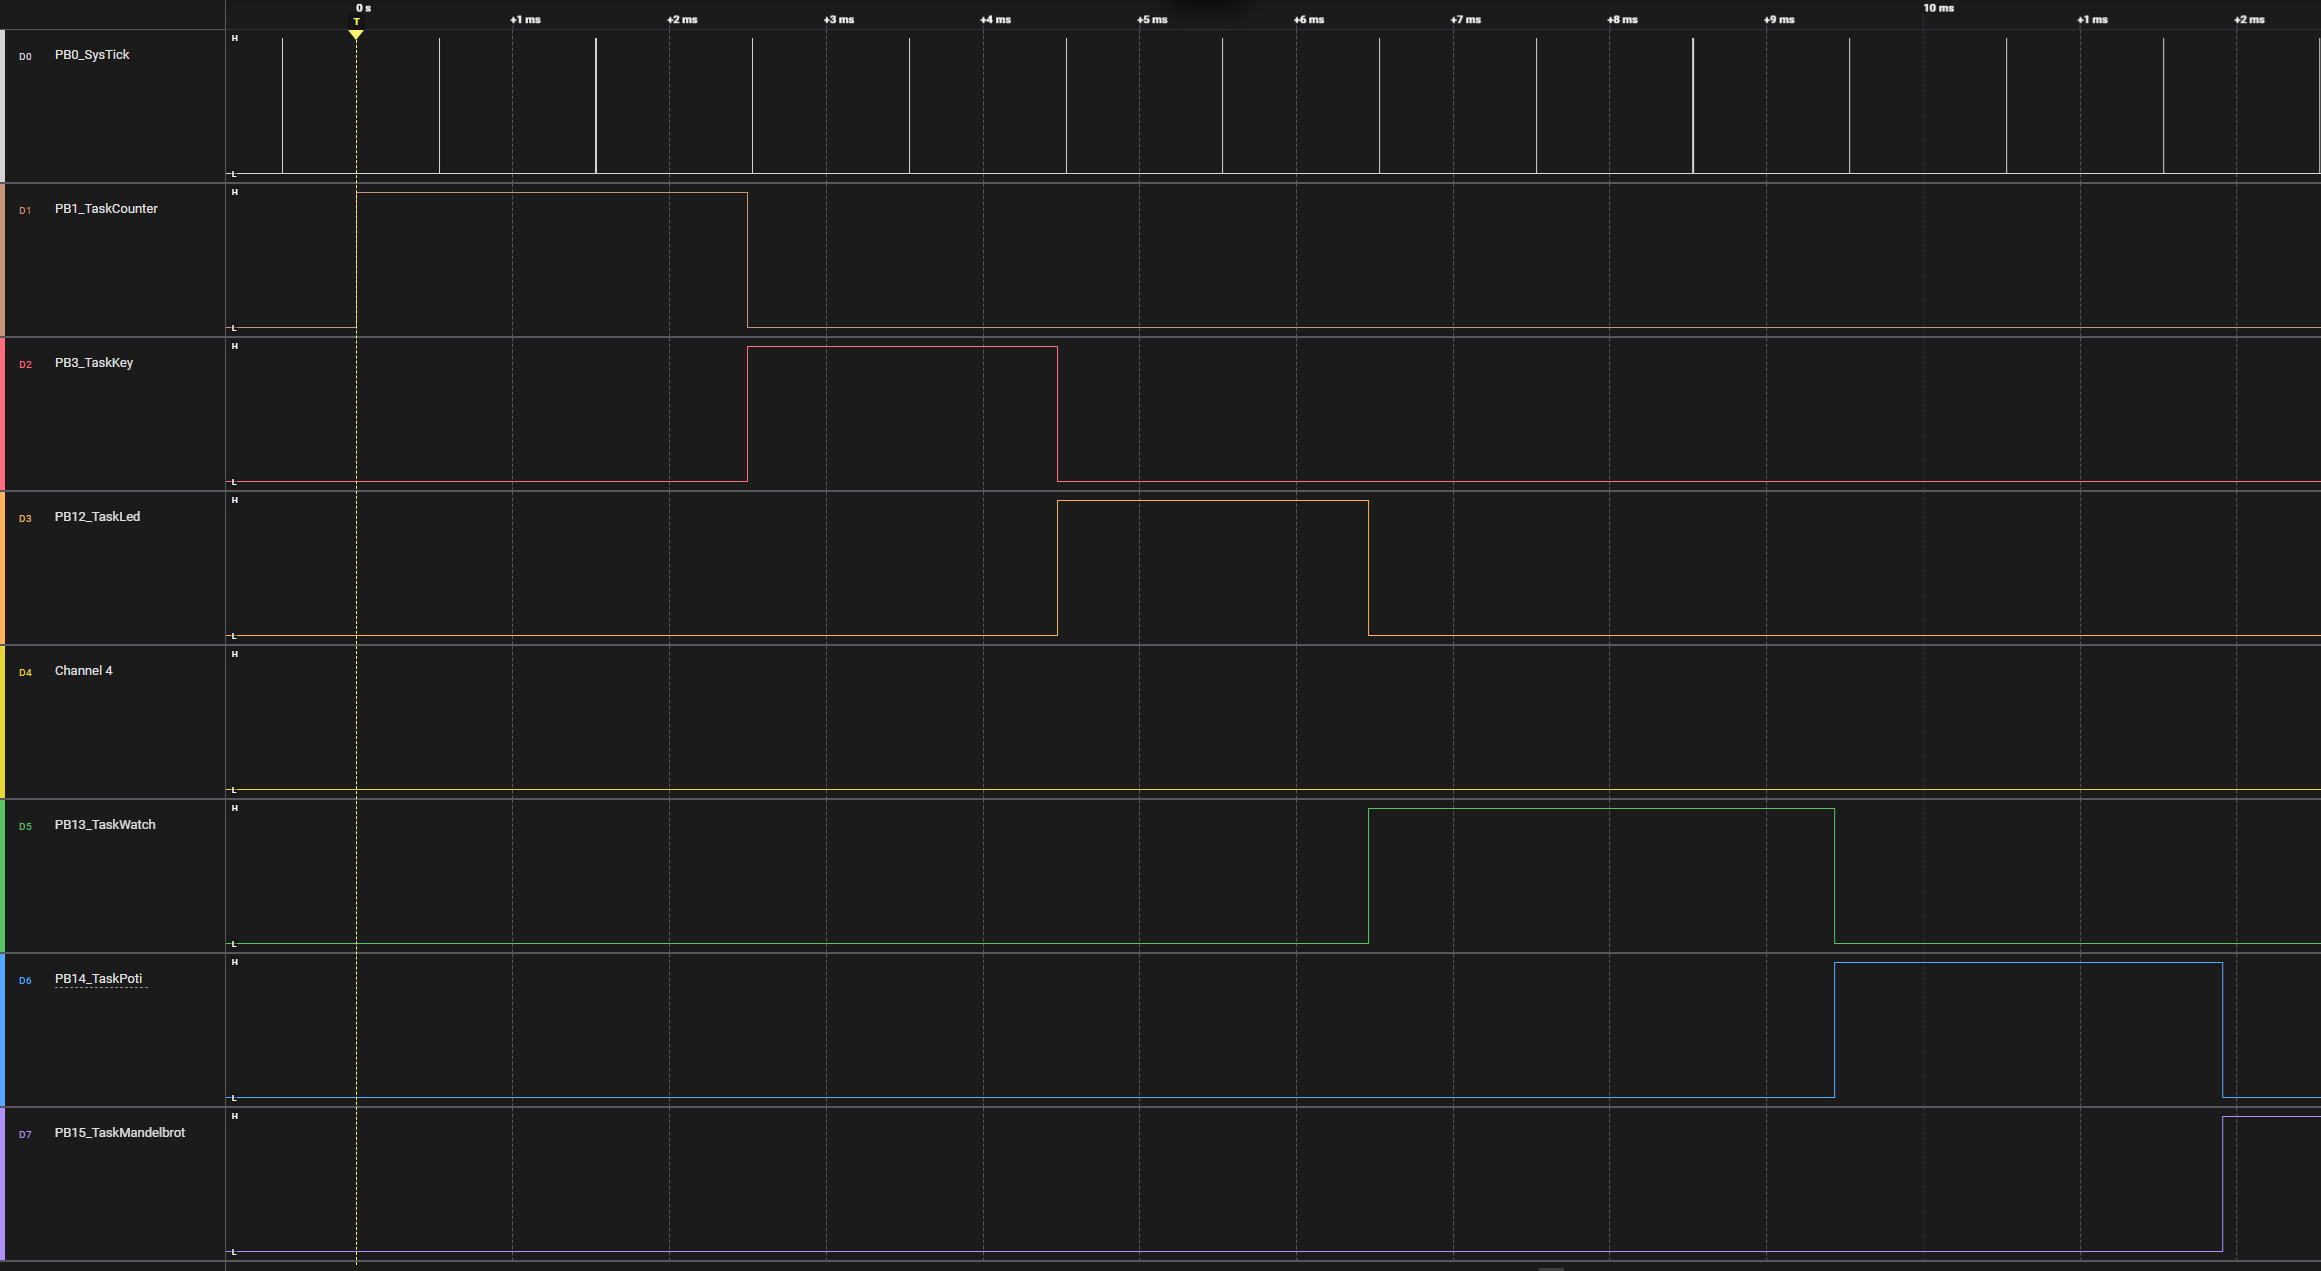
\includegraphics[width=\textwidth]{Images/all_sigs.png}
In der Grafik ist gut zu sehen wie die Tasks nach und nach ausgeführt werden.
Die jeweilige Laufzeit der initialen Tasks aus Übungsaufgabe A sind folgendermaßen:
\begin{itemize}
    \item PB0 Systemtick: 920 ns
    \item PB1 TaskCounter : 2.494 ms
    \item PB3 TaskKey : 1.981 ms
    \item PB12 TaskLed : 1.981 ms
    \item PB13 TaskWatch : 2.971 ms
    \item PB14 TaskPoti : 2.477 ms
    \item PB15 TaskMandelbrot : 16.178 s
\end{itemize}

Um den Overhead der Messungen zu bestimmen wurde einerseits ein mittels Debug\_SwitchDebugPin() im Code direkt hintereinander ein und ausgeschaltet.
Dies wurde mittels Saleae vermessen:
\begin{lstlisting} 
Debug_SwitchDebugPin(DEBUG_PIN_TASKCOUNTER, Bit_SET);
Debug_SwitchDebugPin(DEBUG_PIN_TASKCOUNTER, Bit_RESET);
\end{lstlisting}
Der durch die Messung bestimmte Overhead beträgt 796ns, was ungefähr 38 Zyklen beträgt.
Ein Zyklus entspricht 1/48MHz = 20.883ns
Somit 796ns/20.883ns = 38.2 Cycles. \\

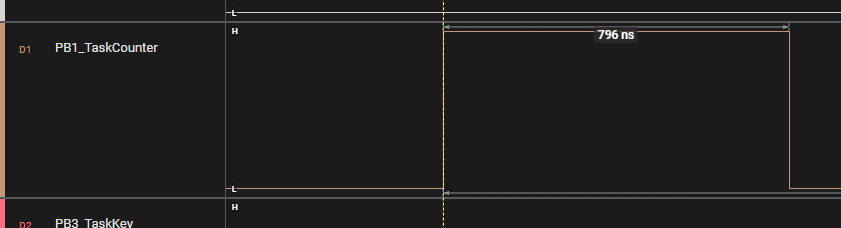
\includegraphics[width=\textwidth]{Images/overhead.png}


\section{Übungsaufgabe B}
Alle Funktionen wurden wie verlangt umgesetzt:
\begin{itemize}
    \item Der Zahlenwert im rechts-oberen Eck des Displays aktualisiert sich mit jedem Counter-Aufruf.
    \item Die Keys Setzen die Schriftfarbe und die Farbe der zur Zeit gezeichneten Pixel des Mandelbrot Diagramms entweder zu Schwarz(WAKE-UP), Blau(USER0) oder Gelb(USER1). 
    \item Die LEDs leuchten abwechselnd alle 100ms.
    \item Die Watch zeigt die Run-Time wie verlangt an.
    \item Die Mandelbrot Funktion zeichnet das Diagramm in der unteren Hälfte des Displays.
\end{itemize}
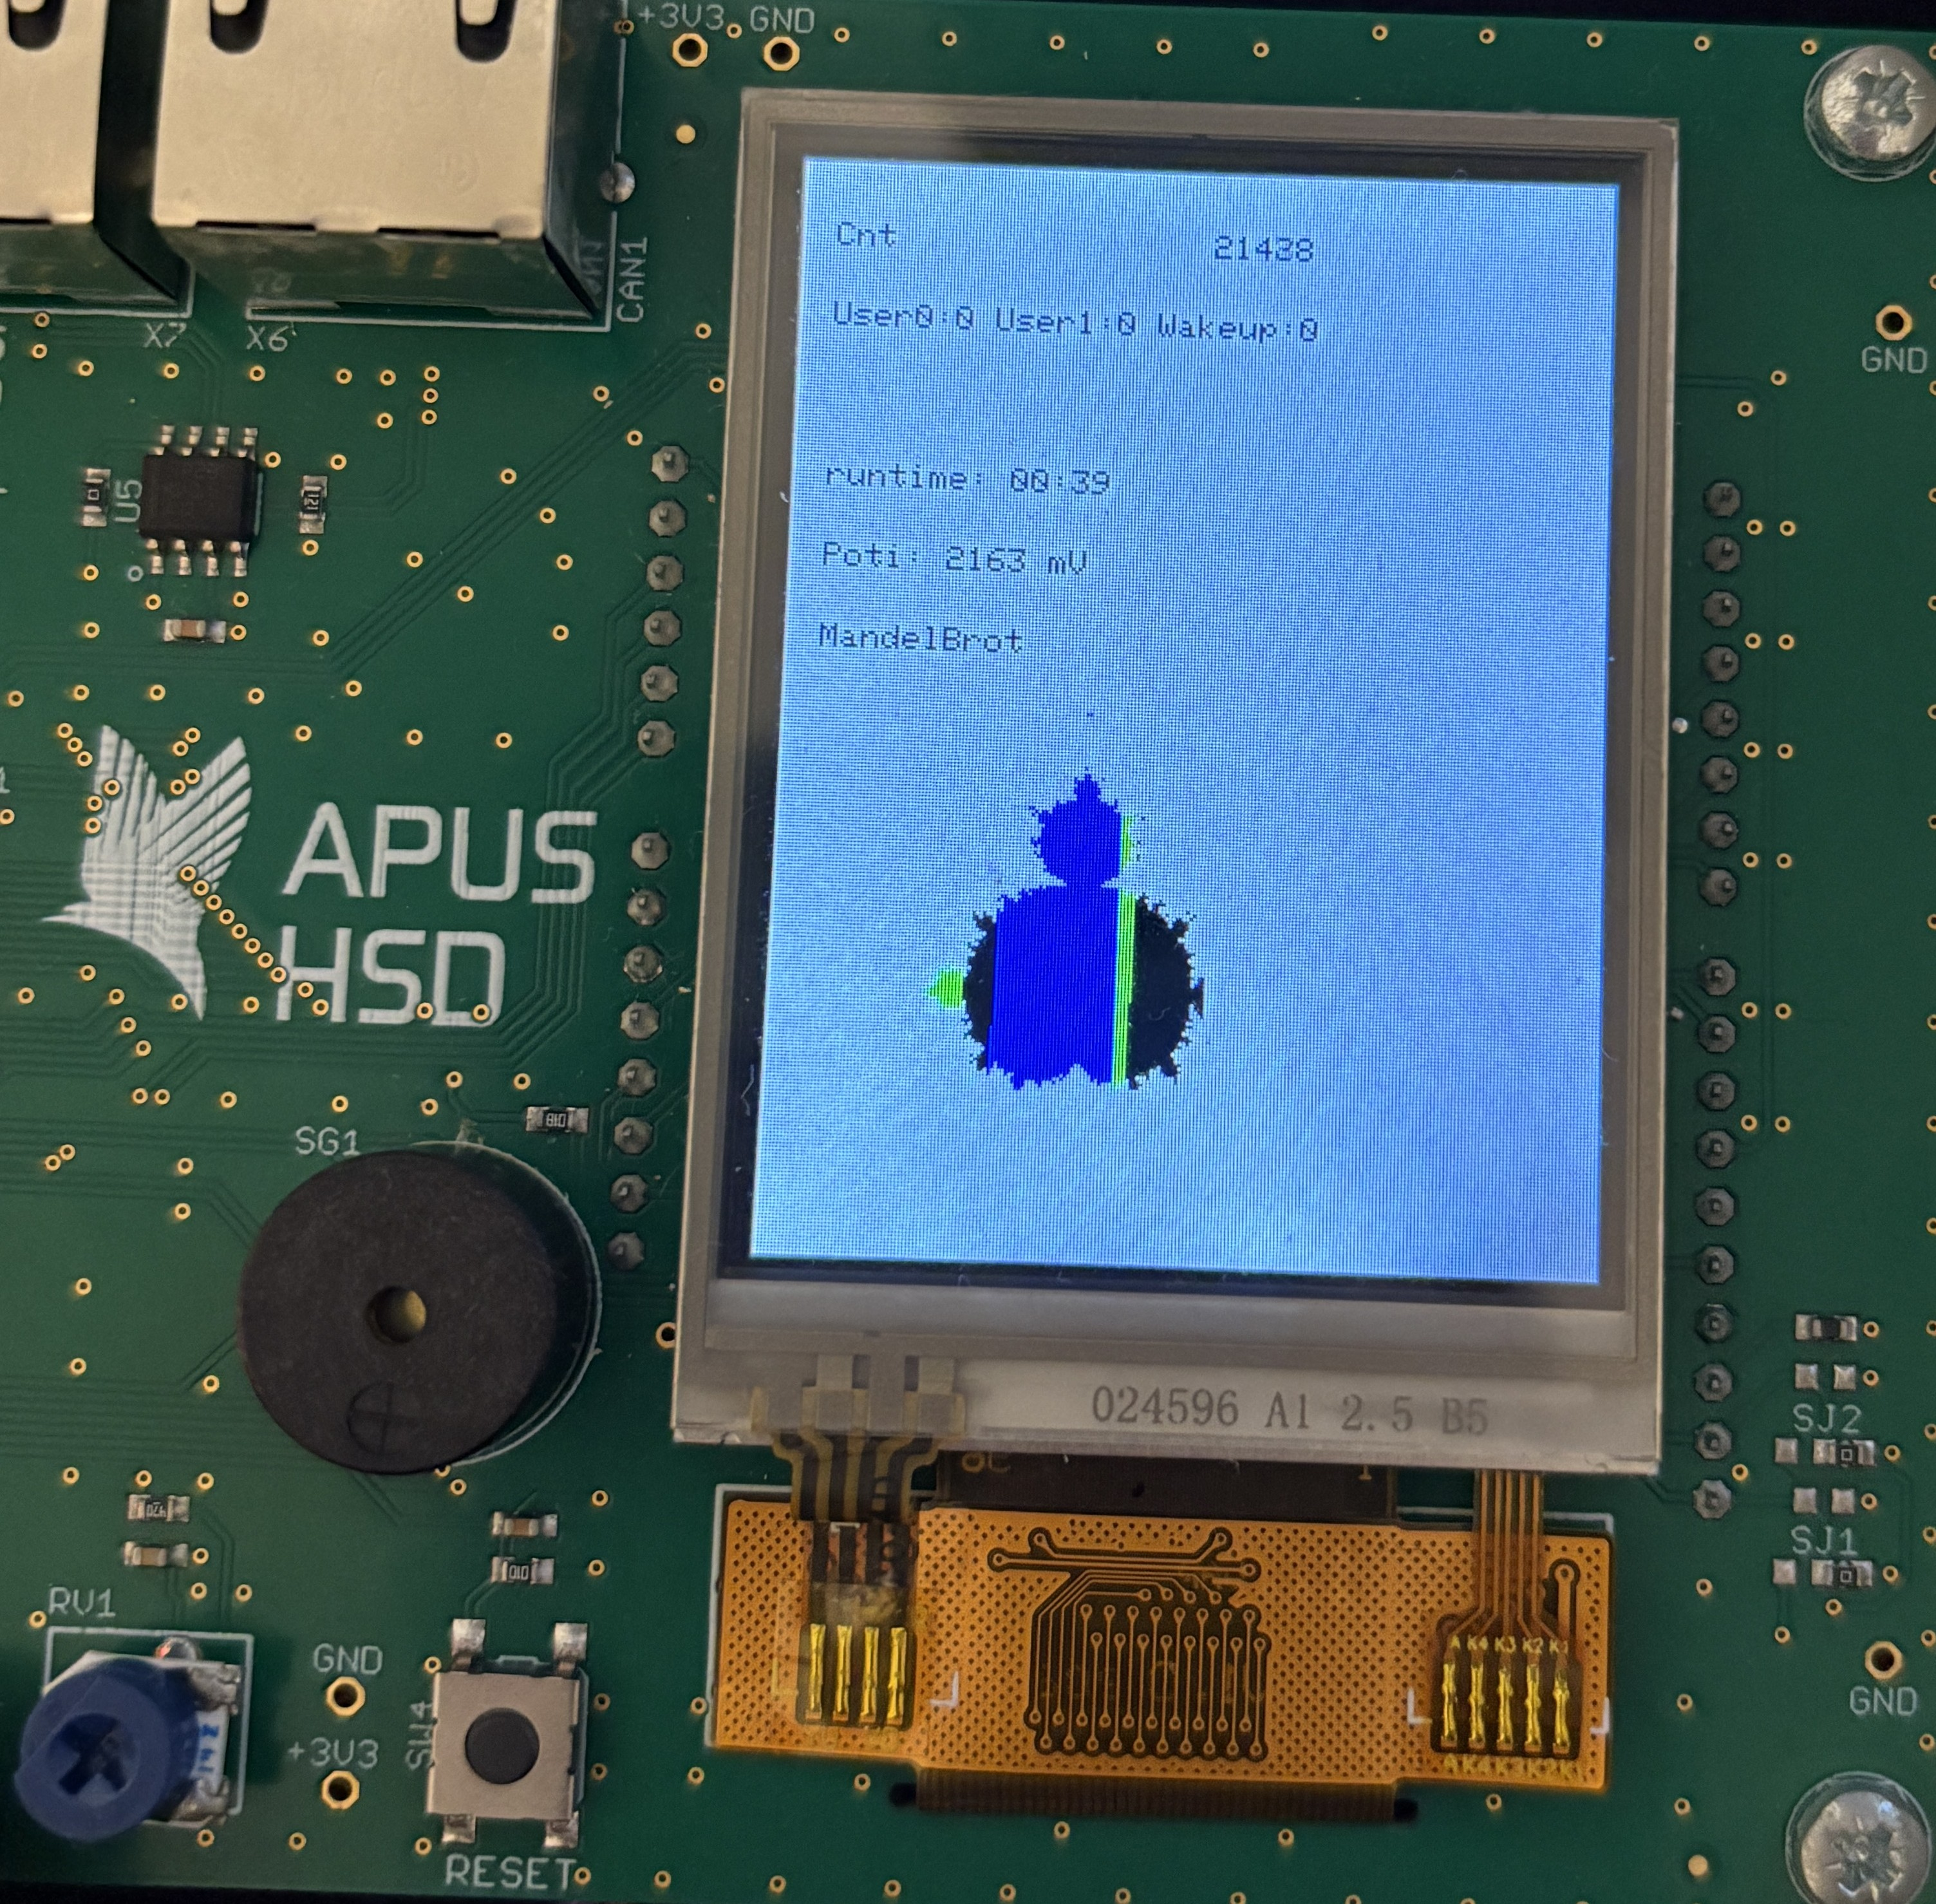
\includegraphics[width=\textwidth]{Images/IMG_5660.JPG}
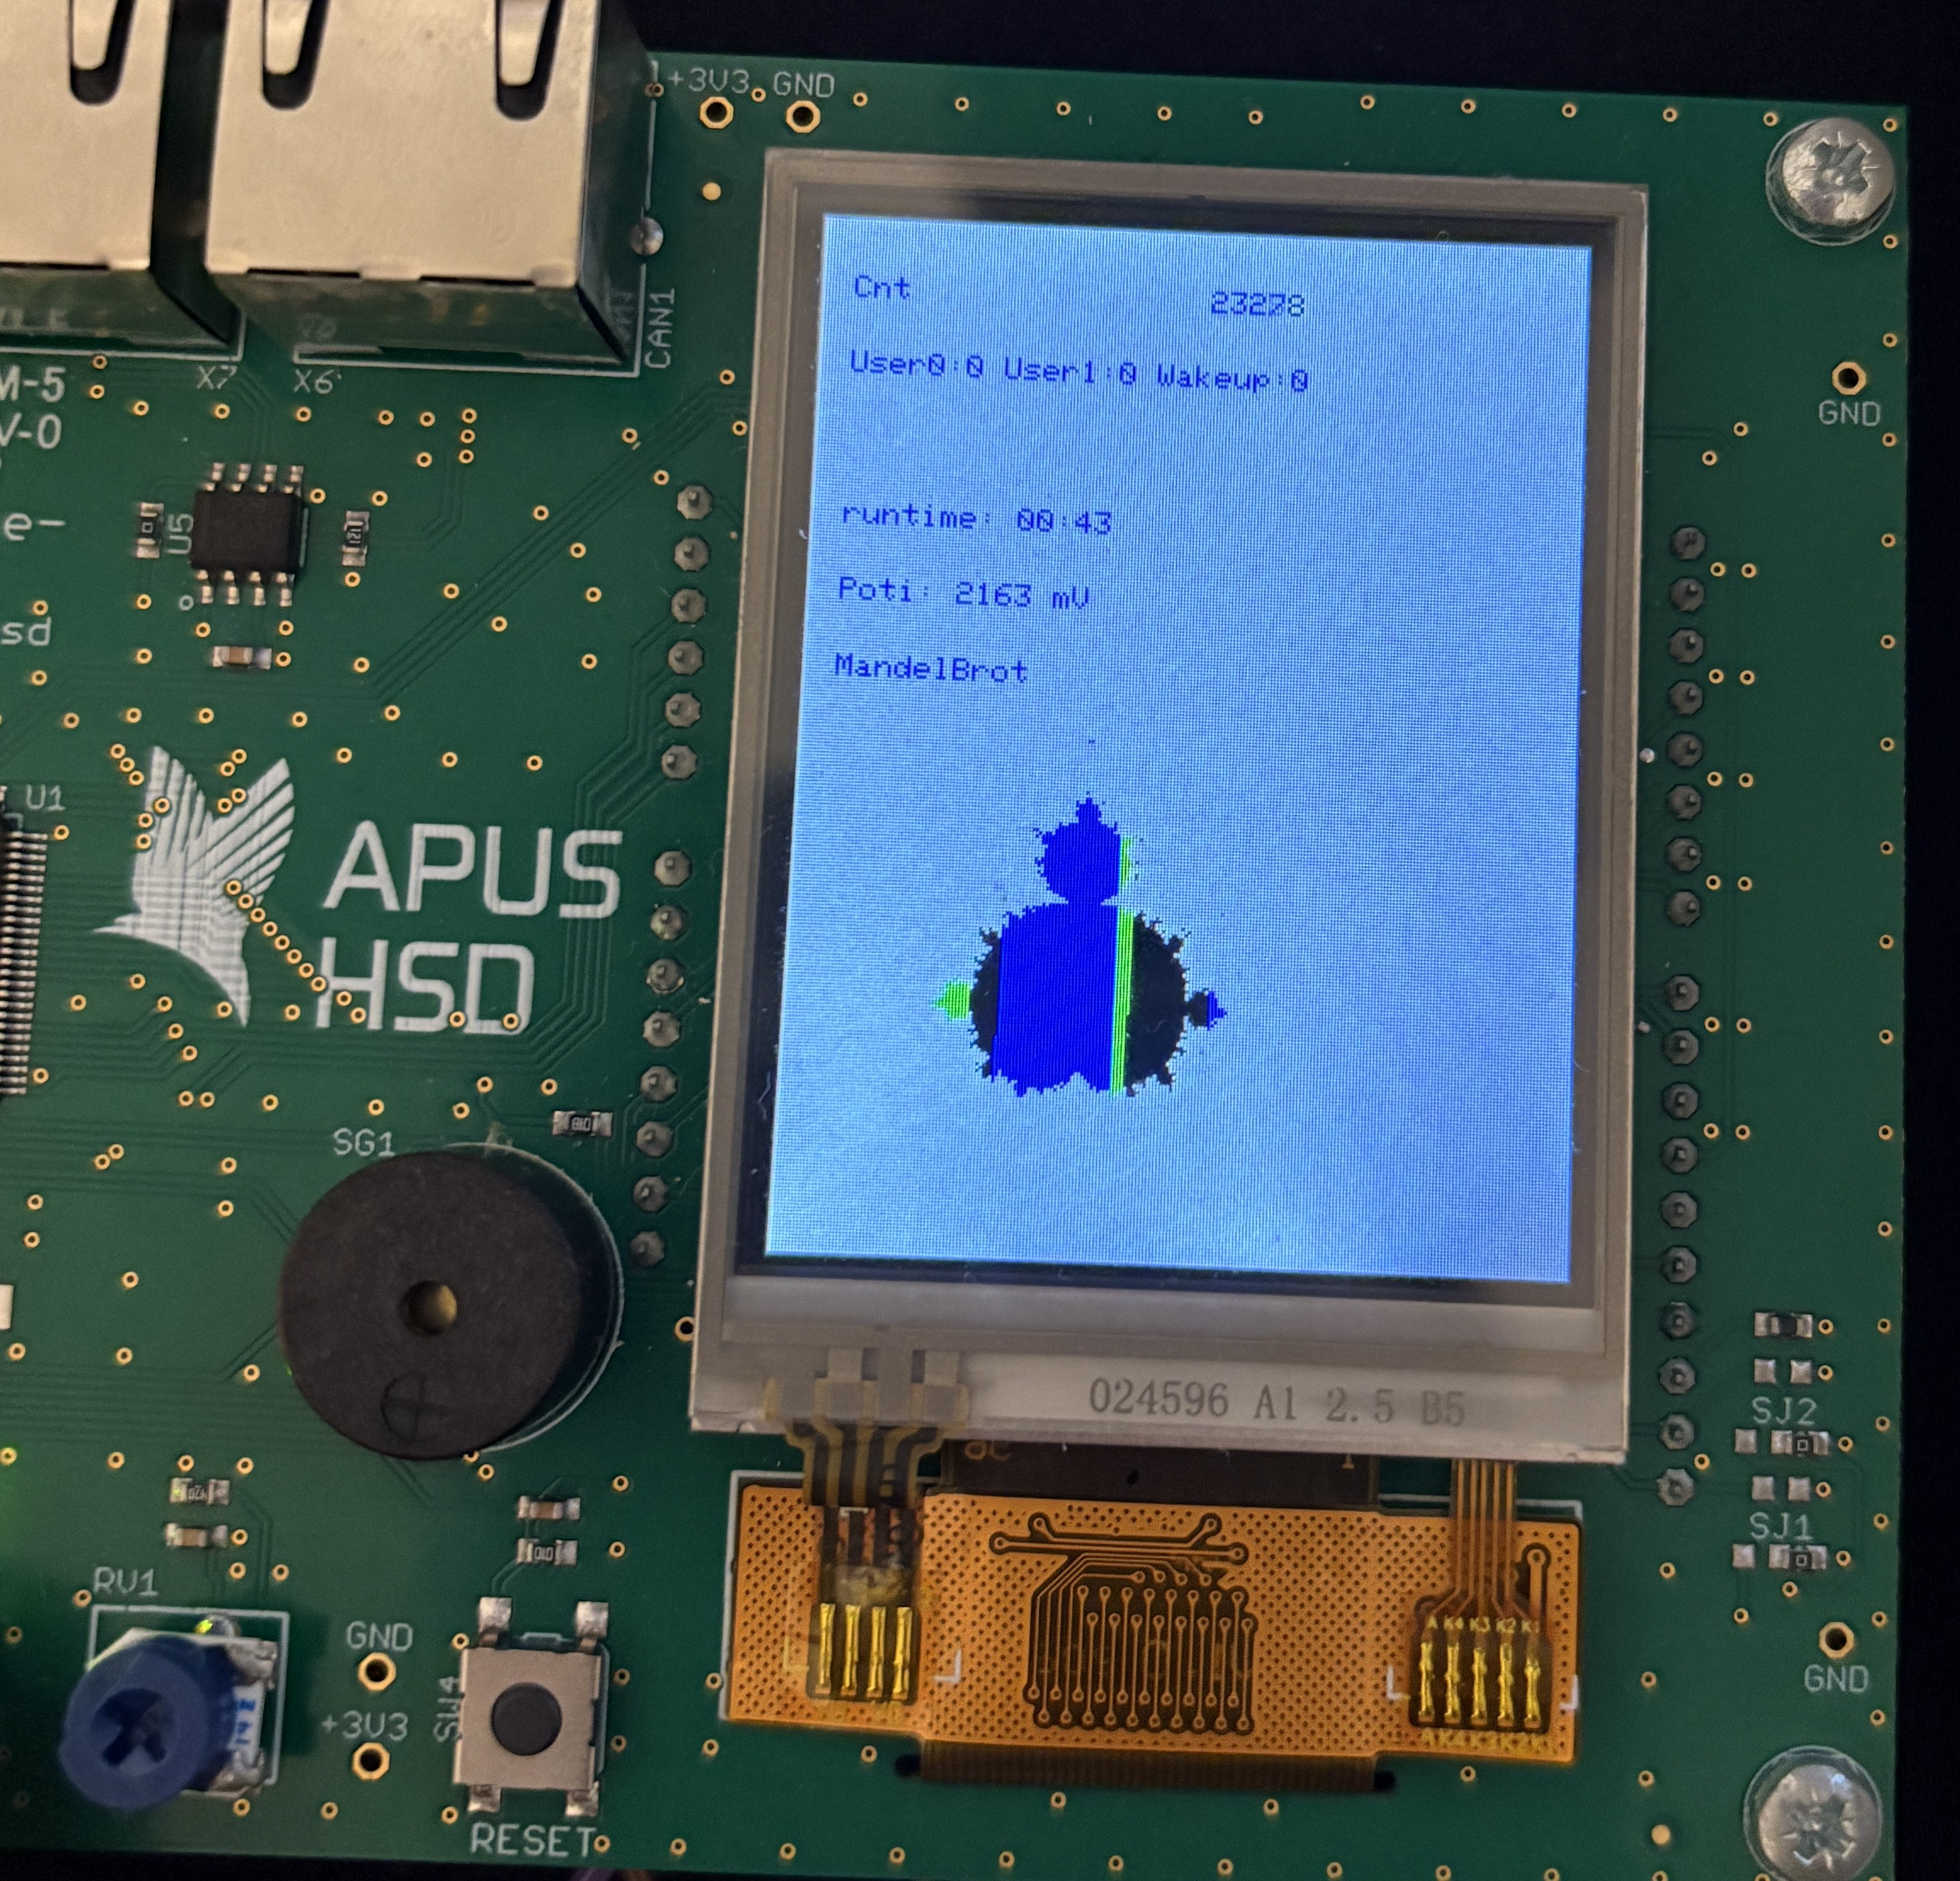
\includegraphics[width=\textwidth]{Images/IMG_5661.JPG}
\\
\\
Um die Tasks alle so reaktiv wie verlangt ausführen zu können wurde auf ko-operatives Scheduling gesetzt.
Mithilfe des Systicks wird ein Zeitdelta berechnet, um festzustellen, wie lange die jeweiligen Tasks laufen.
Das Scheduling nutzt diese Zeitdeltas, um festzustellen, ob ein Task an der Reihe ist oder an andere Tasks freigeben sollte.
\\
\\
Mithilfe von defines werden die Zeitschlitze definiert, in welchen ein Task vorkommen muss.
Die Priorisierung erfolgt dabei durch eine If-else-if-Kette, wobei der TaskCounter() die höchste Prio erhält.

\begin{lstlisting} 
if (lastCounter >= TASK_SCHEDULER_COUNTER) {
    Debug_SwitchDebugPin(DEBUG_PIN_TASKCOUNTER, Bit_SET);
    TaskCounter();
    Debug_SwitchDebugPin(DEBUG_PIN_TASKCOUNTER, Bit_RESET);
    lastCounter = 0;
}
else if (lastKey >= TASK_SCHEDULER_KEY) {
    ...
}
else if (lastPoti >= TASK_SCHEDULER_POTI) {
    ...
}
    ...
\end{lstlisting}

Dieses Scheduling betrifft hauptsächlich den Mandelbrot-Algorithmus, da dieser bis zu 17s andauern kann.
Hierzu wurde die Mandelbrot Funktion so zerlegt, sodass der Algorithmus immer nur für einen definierten Rechnenschritt ausgeführt wird.
Die x und y Koordinaten der Rechenschritte wurden dazu zu Static-Variablen geändert, wodurch der Rechenschritt beim Austrete aus der Funktion beibehalten wird.
Der längste Rechenschritt des Mandelbrot-Algorithmus dauert hierbei laut Messung maximal 3.5ms.
\\
\\
Der Mandelbrot-Algorithmus erhält die geringste Priorität in der Scheduling-Kette und wird nur ausgeführt, wenn kein anderer Task laufen muss.
Dabei wird auch darauf geachtet, dass der Algorithmus nur dann läuft, wenn keine andere Funktion in weniger als 4ms an der Reihe wäre,
 da die Mandelbrot-Funktion ansonsten in den Zeitschlitz der höher-prioren Funktion eindringen würde.

\begin{lstlisting}
// determine if mandelbrot can run or if mandelbrot should wait until next timeslot
else if( 
    (TASK_SCHEDULER_COUNTER - lastCounter) > MANDELBROT_OVERHEAD
    &&(TASK_SCHEDULER_KEY - lastKey) > MANDELBROT_OVERHEAD 
    ...
) {
    // if no other task executed: mandelbrot
    ...
\end{lstlisting}

\subsection{Alle gemessenen Zeiten der Übungsaufgabe B}

Alle gemessenen Maximalzeiten zwischen den Aufrufen der Funktionen:
\begin{itemize}
    \item PB1 TaskCounter : 19.62ms
    \item PB3 TaskKey : 49.668ms
    \item PB12 TaskLed : 99.52ms
    \item PB13 TaskWatch : 999.846ms
    \item PB14 TaskPoti : 49.668ms
    \item PB15 TaskMandelbrot : Dauer um die 20s
\end{itemize}

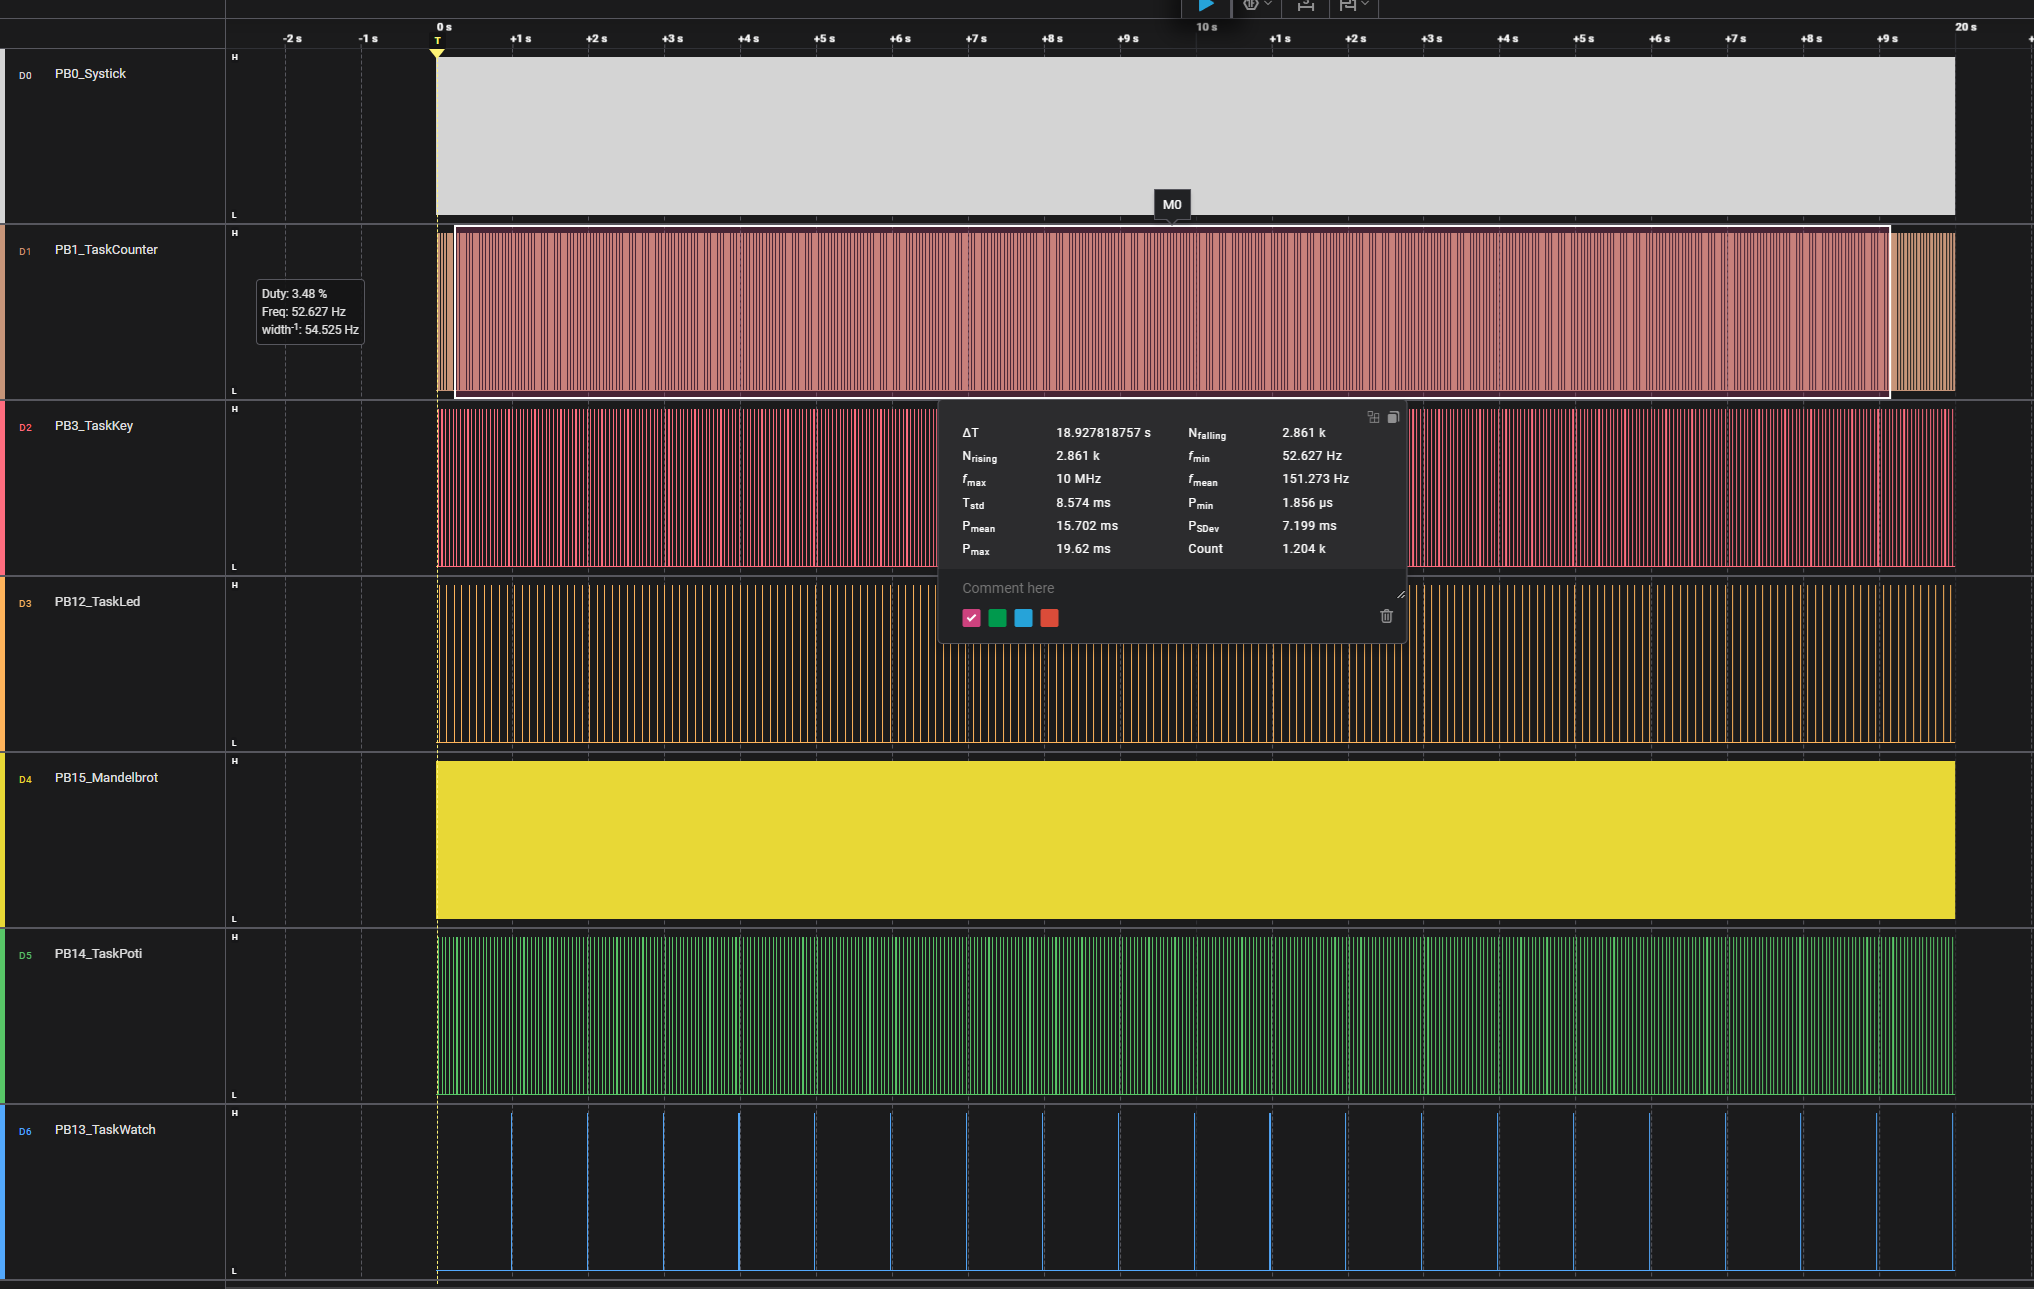
\includegraphics[width=\textwidth]{Images/TaskCounterAVG.png}
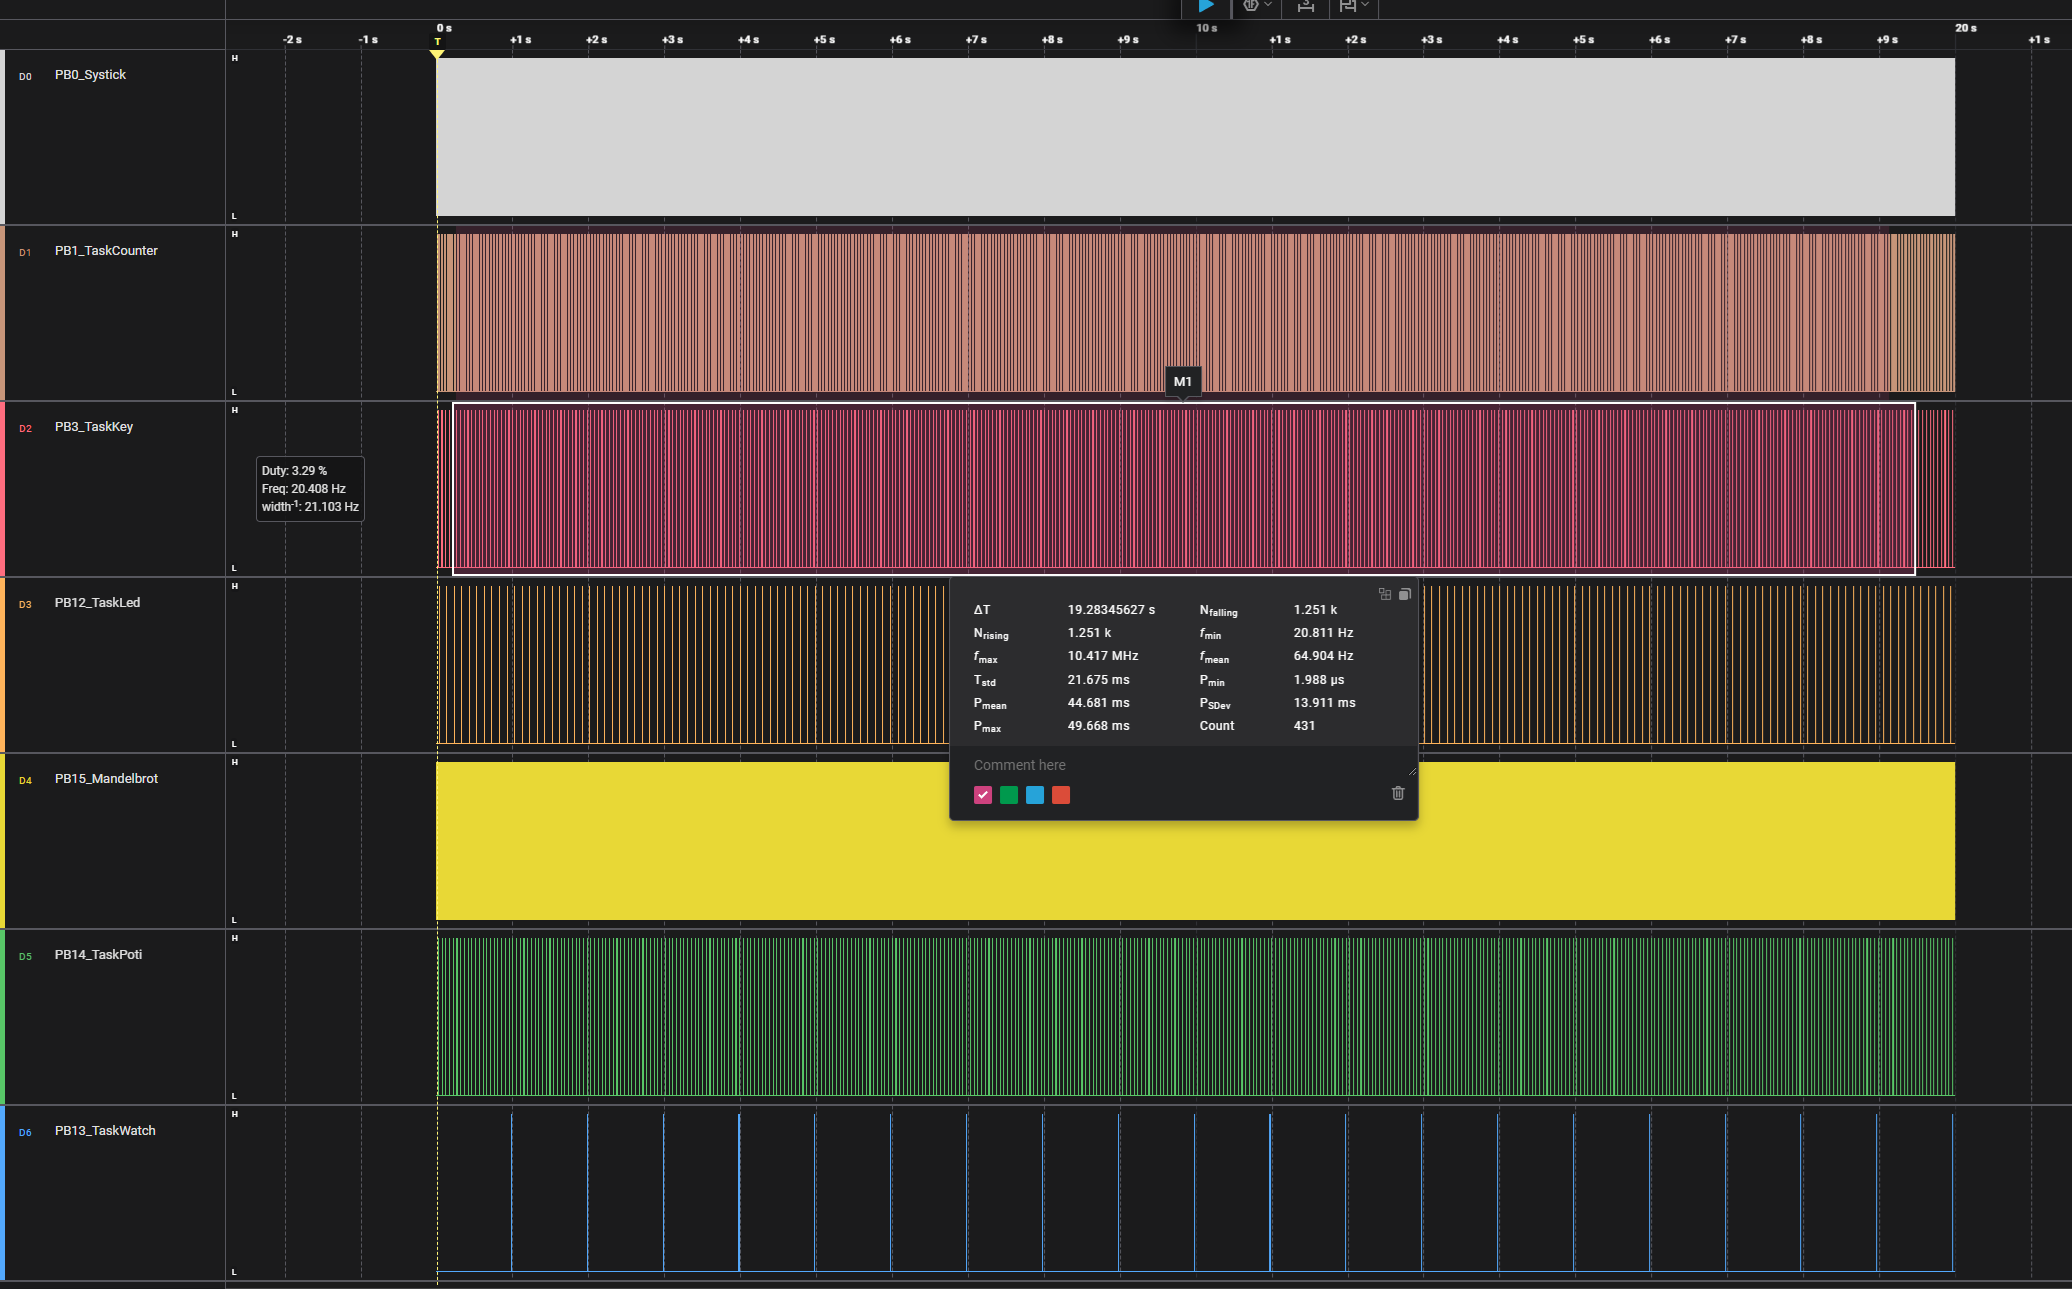
\includegraphics[width=\textwidth]{Images/TaskKey_AVG.png}
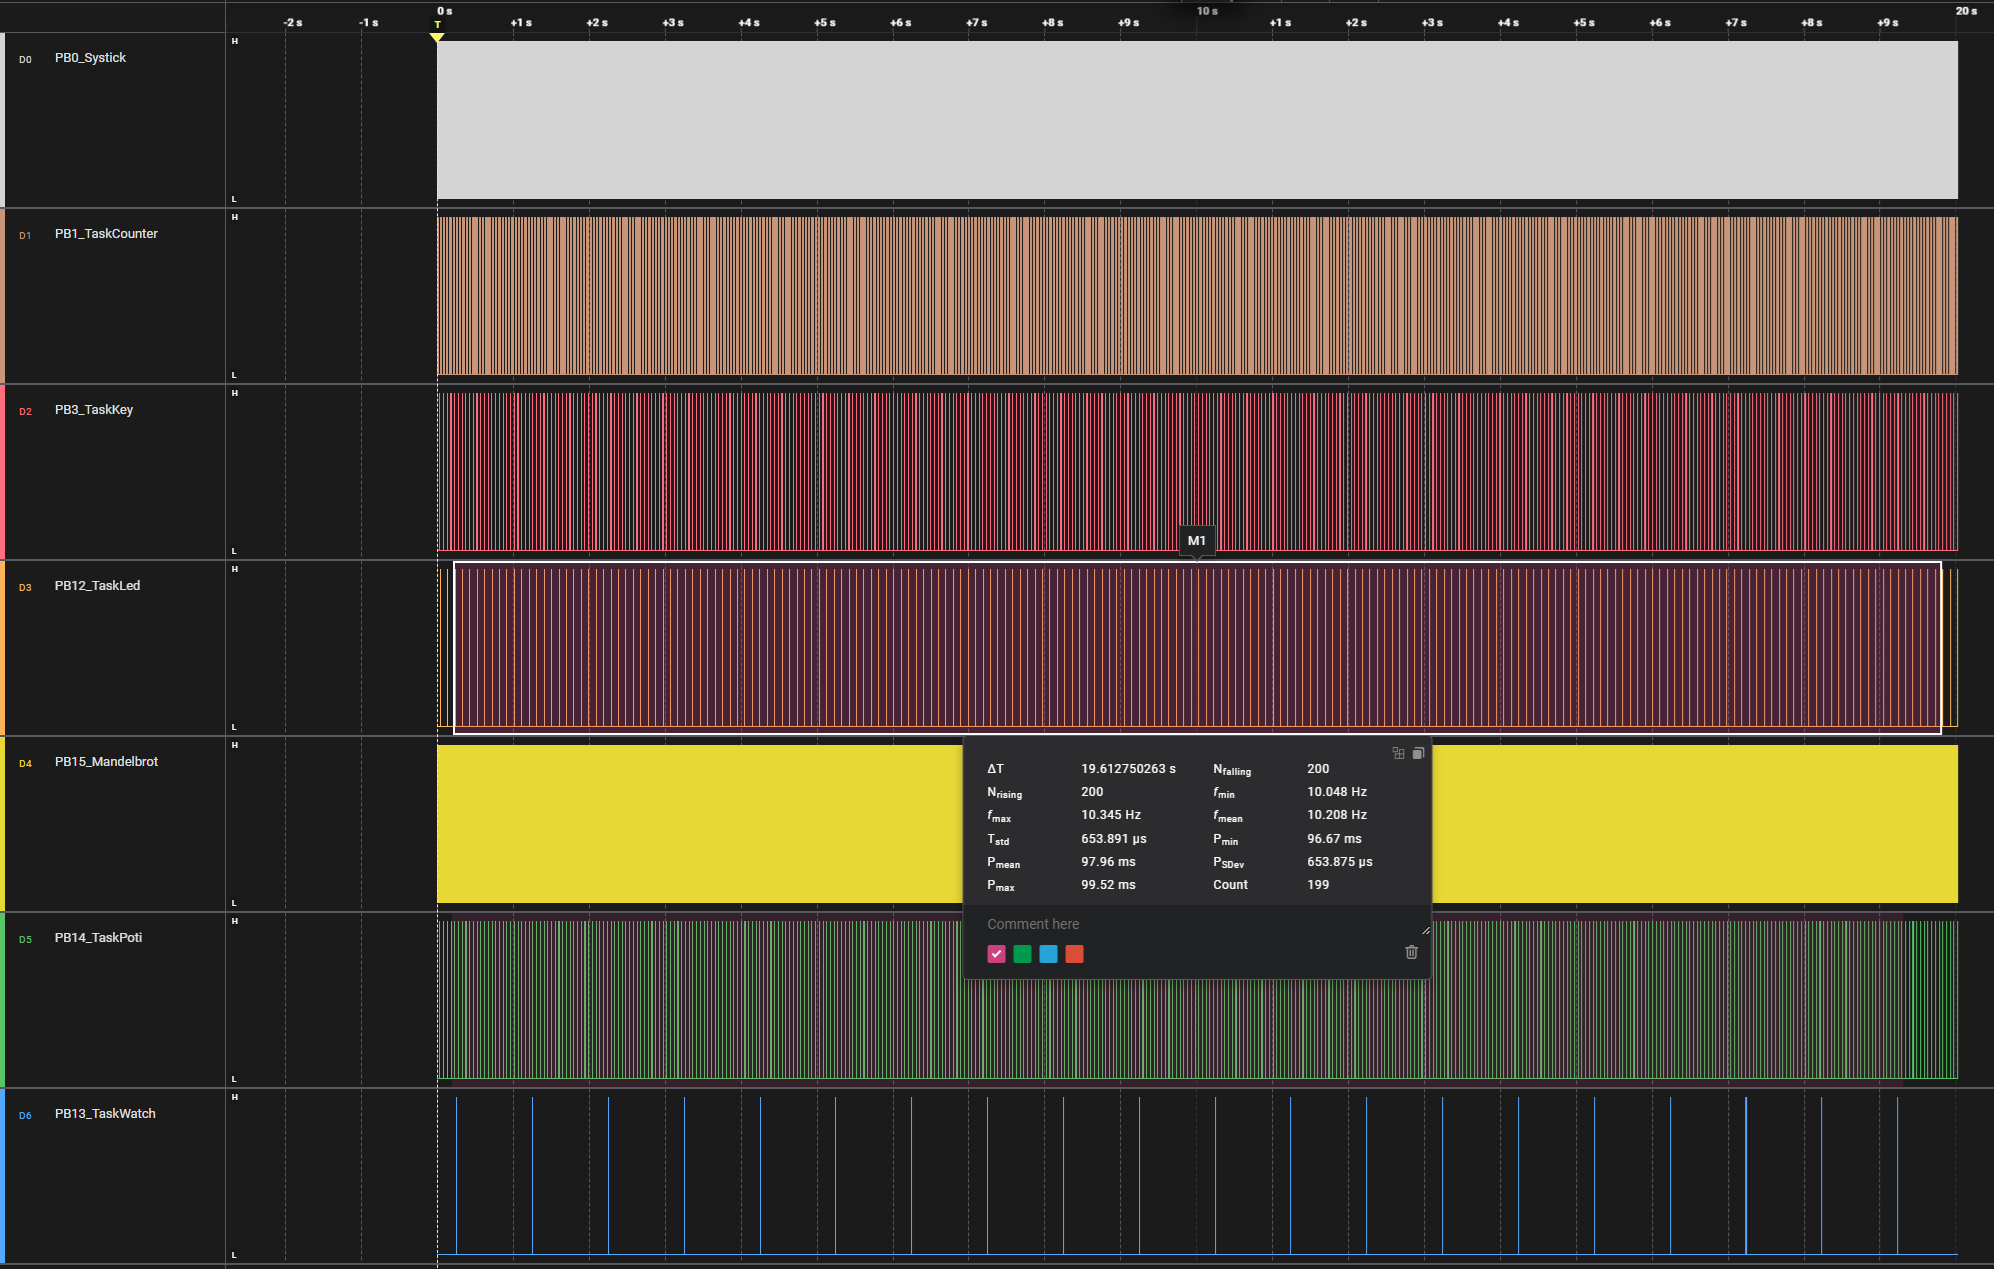
\includegraphics[width=\textwidth]{Images/TaskLed_AVG.png}
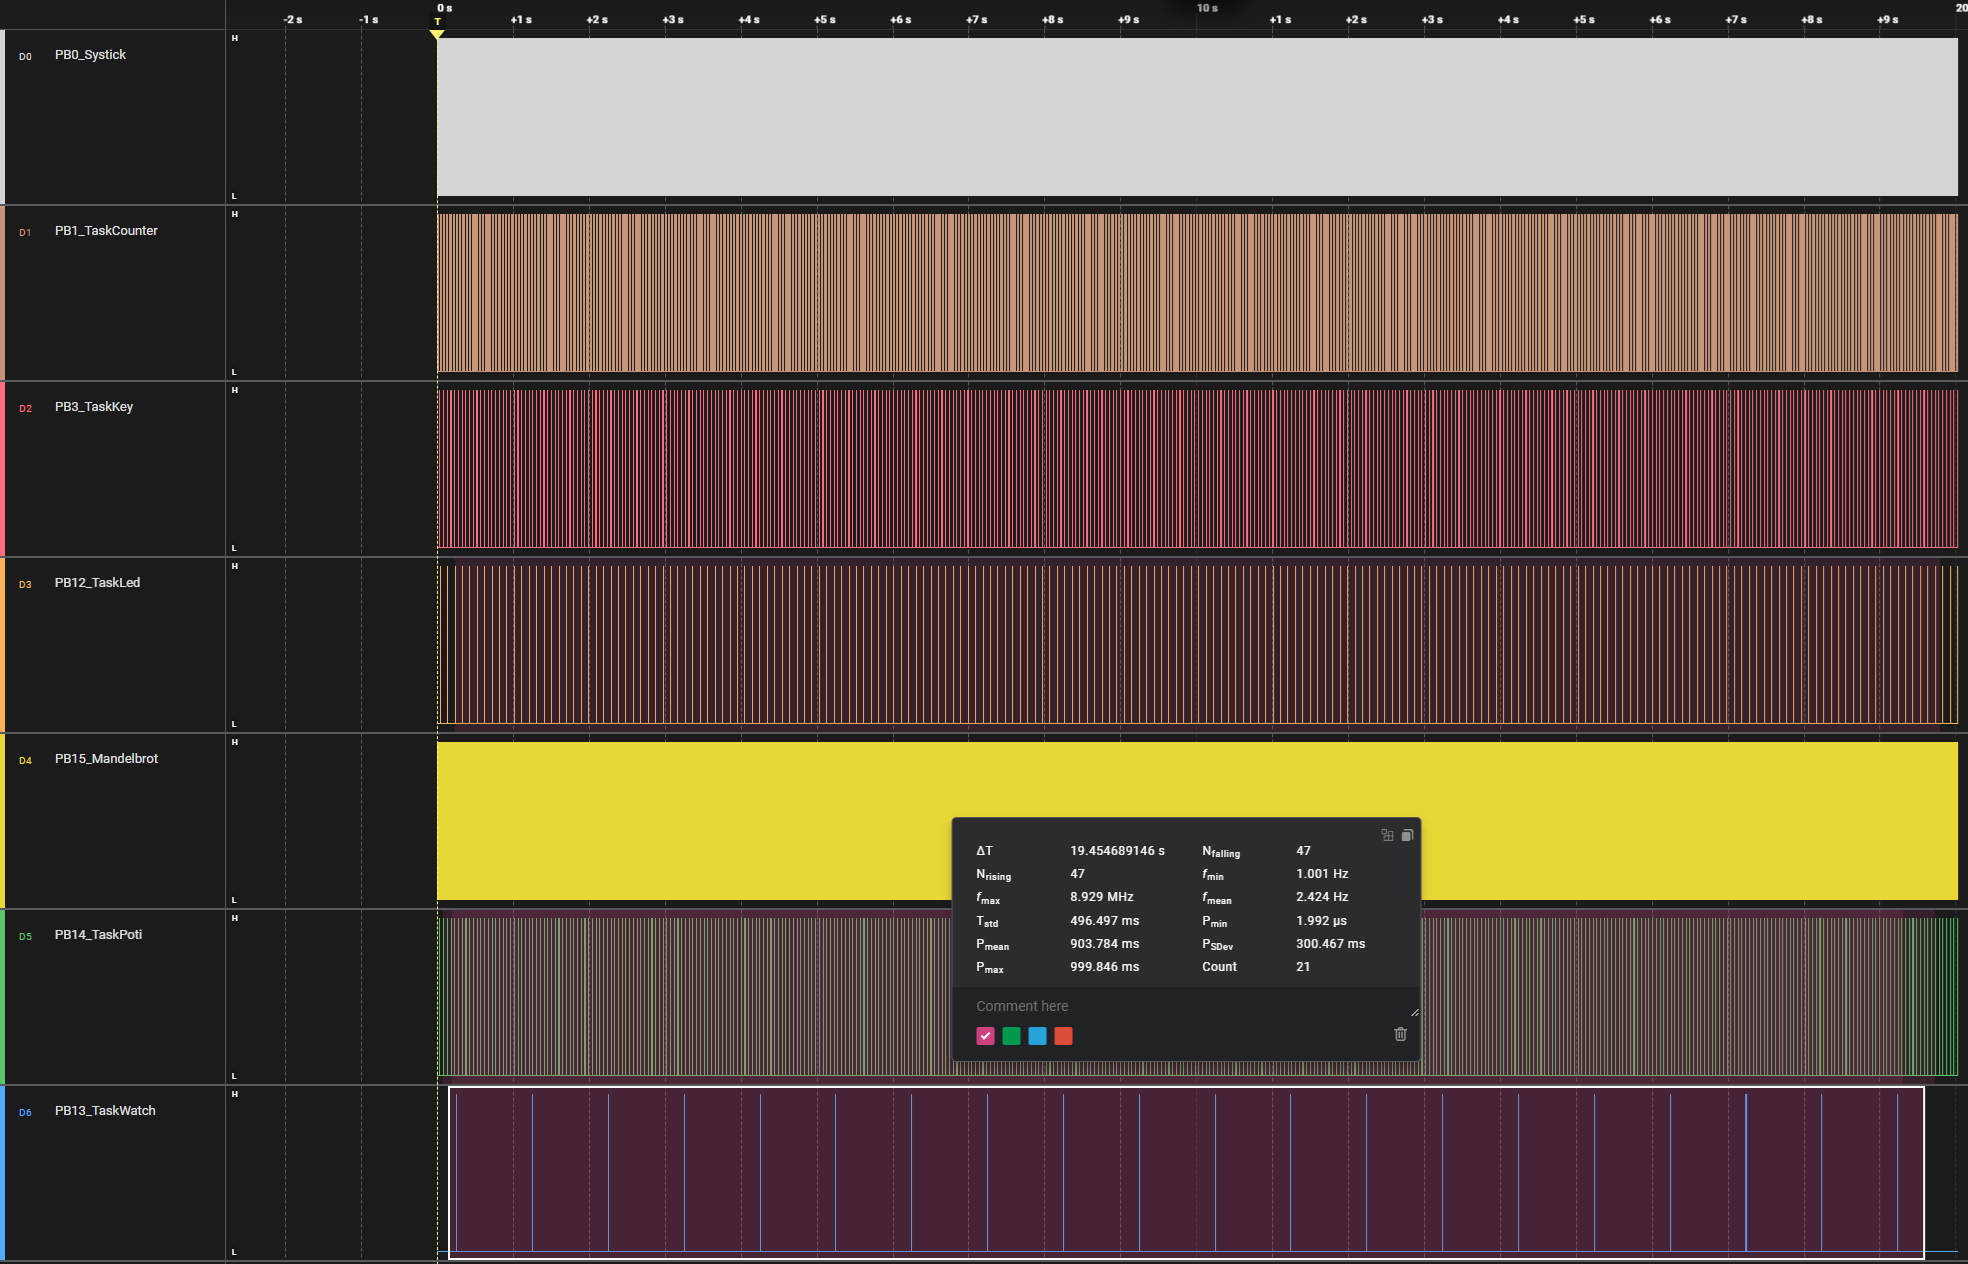
\includegraphics[width=\textwidth]{Images/TaskWatch_AVG.png}
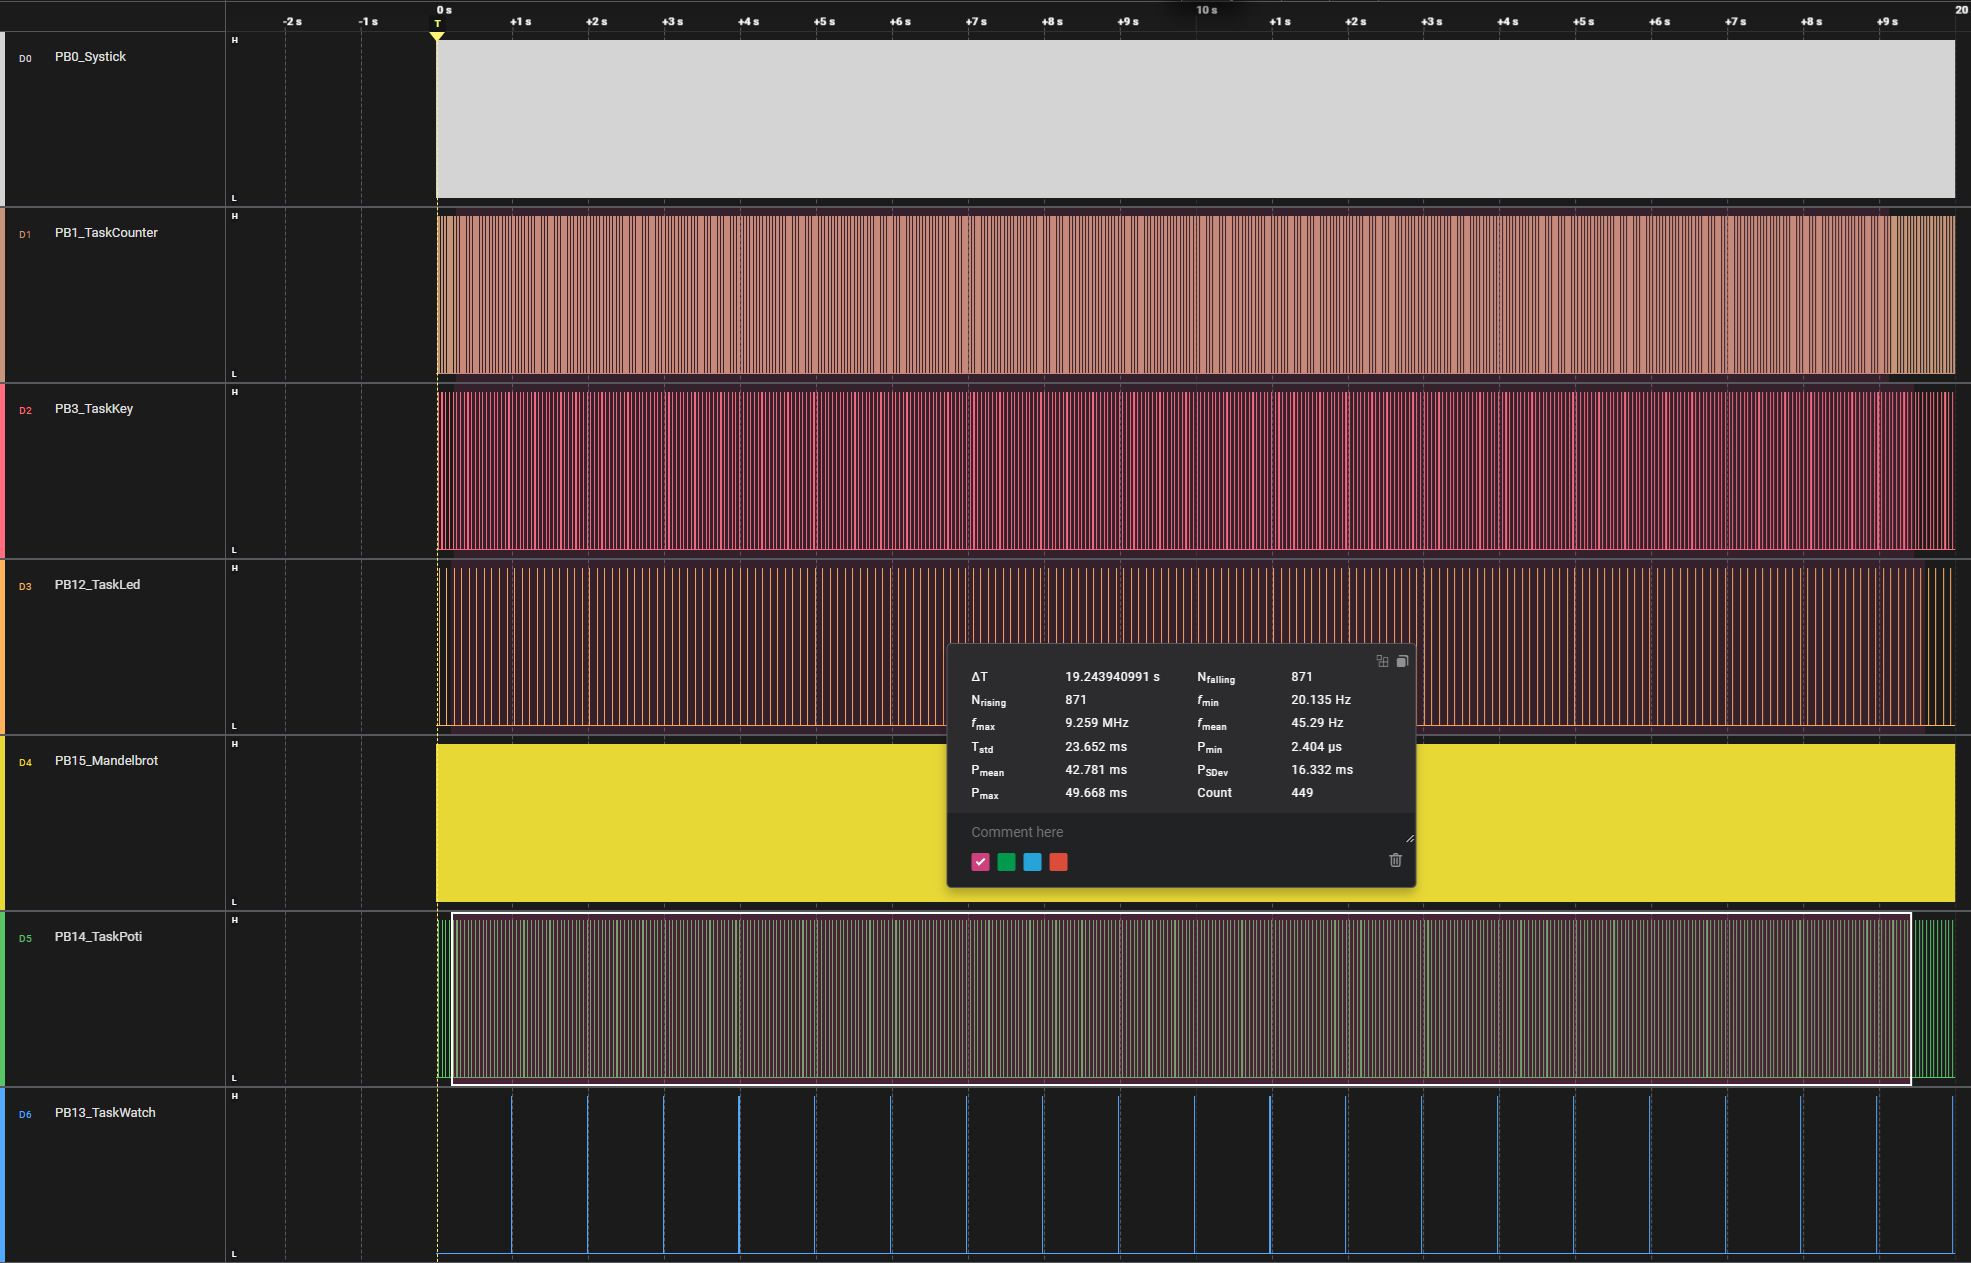
\includegraphics[width=\textwidth]{Images/TaskPoti_AVG.png}
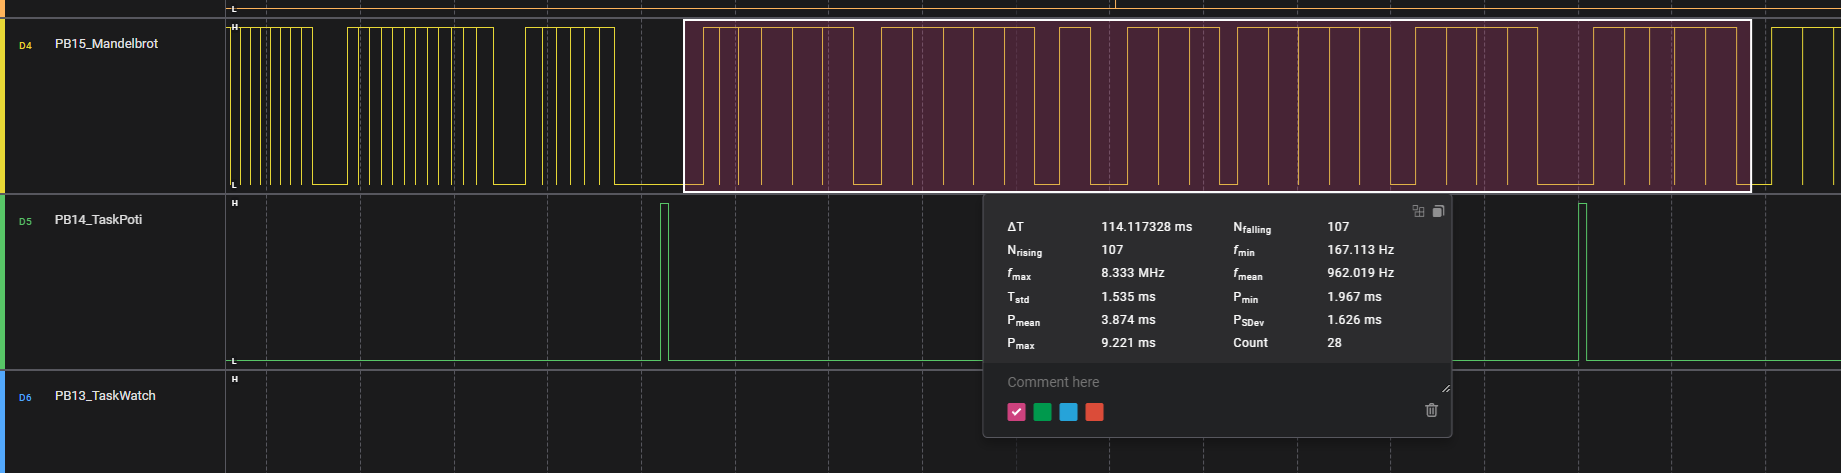
\includegraphics[width=\textwidth]{Images/TaskMandelbrot_AVG.png}

\clearpage
\section{Übungsaufgabe C}
Die Initialisierung aller ISRs und aller Ressourcen wird noch auf dem Master-Stack durchgeführt.
Da alle Anwendungen in der Superloop im Main laufen wird davor auf den Process-Stack geschaltet.
Somit laufen alle Anwendungen auf dem Process-Stack.

\begin{lstlisting}
// global static for psp
static uint32_t taskStack[512];

int main(void) {
    ...
    __set_PSP((uint32_t)(taskStack + 512)); // set psp to size
    __set_CONTROL(0x02);                    // switch to psp
    __ISB();                                // clear pipeline

    while (1) {
        ...
    }
\end{lstlisting}

Die sinnvollste Aufteilung ergibt sich aus der Ausführung aller Tasks im Process-Stack.
Systick und andere Prozesse, welche den Interrupt nutzen, werden nämlich immer mittels Master-Stack ausgeführt.
Somit wird getrennt zwischen Anwendungen, wie beispielsweise dem Mandelbrot-Algorithmus und den Interrupt-Serviceroutinen.

\subsection{Analyse}
Durchgeführt wird der Switch durch das setzten des PSP, das Schreiben auf das CONTROL Register mit MSR und das Flusher Pipeline und laden der neuen Instruktionen mittels ISB:
ISB agiert hier auch als Instruction Synchronisation Barrier.
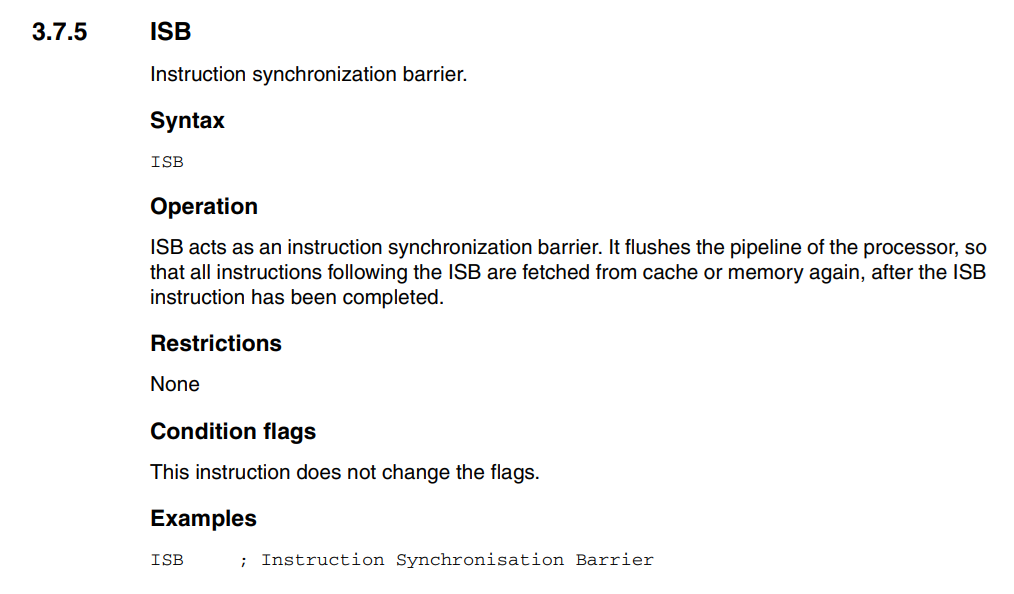
\includegraphics[width=\textwidth]{Images/isb.png}
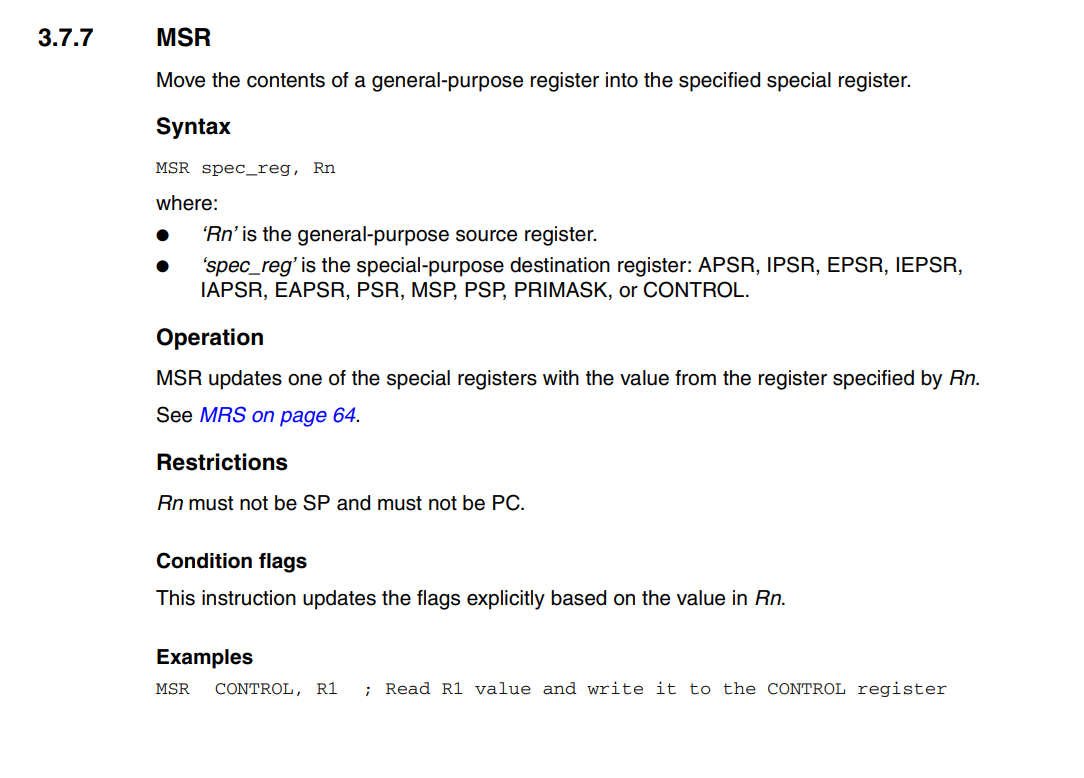
\includegraphics[width=\textwidth]{Images/msr.png}
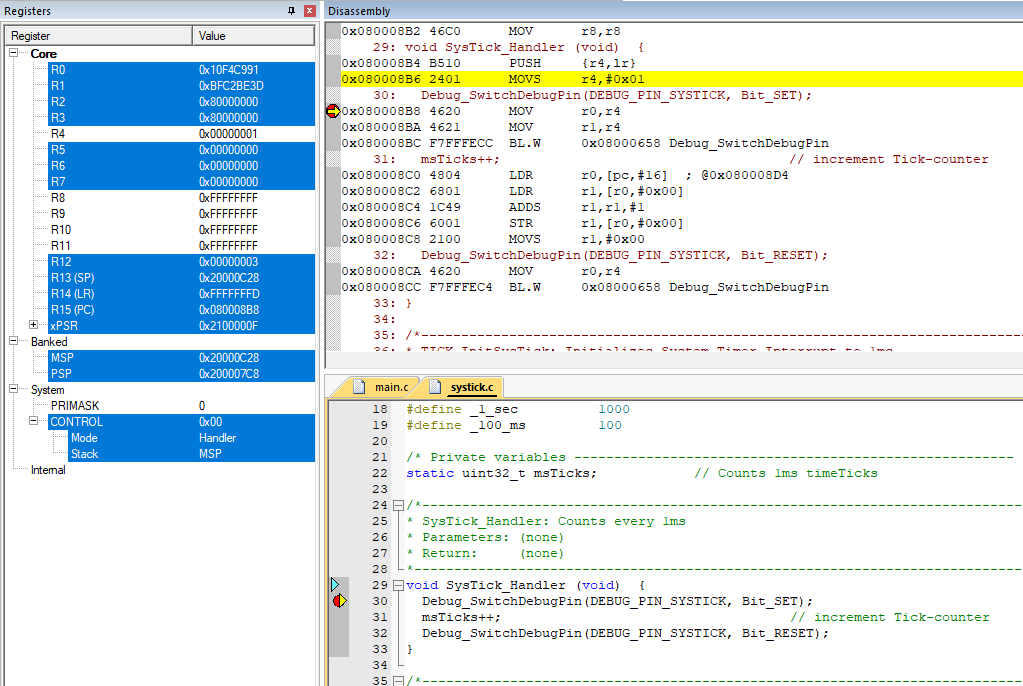
\includegraphics[width=\textwidth]{Images/isr.png}

Zu Beginn läuft der STM32 immer auf dem Master-Stack, der Switch auf den Process-Stack muss immer Manuell erfolgen.
Hier ist zu sehen wie alle inits im device default auf dem Master-Stack ausgefürt werden:
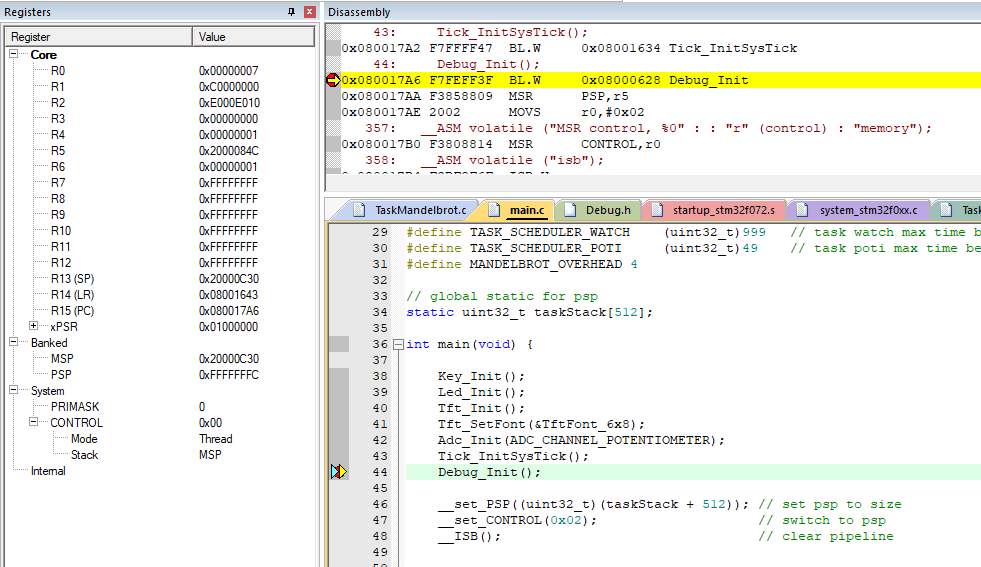
\includegraphics[width=\textwidth]{Images/vor_psp.png}
Mithilfe dieser Codezeilen wird ein Switch auf den PSP vor der Super-Loop durchgeführt:
\begin{lstlisting}
__set_PSP((uint32_t)(taskStack + 512)); // set psp to size
__set_CONTROL(0x02);                    // switch to psp
__ISB();                                // clear pipeline
\end{lstlisting}

Hier erkennt man die Initialisierung des PSP im Assembler code:
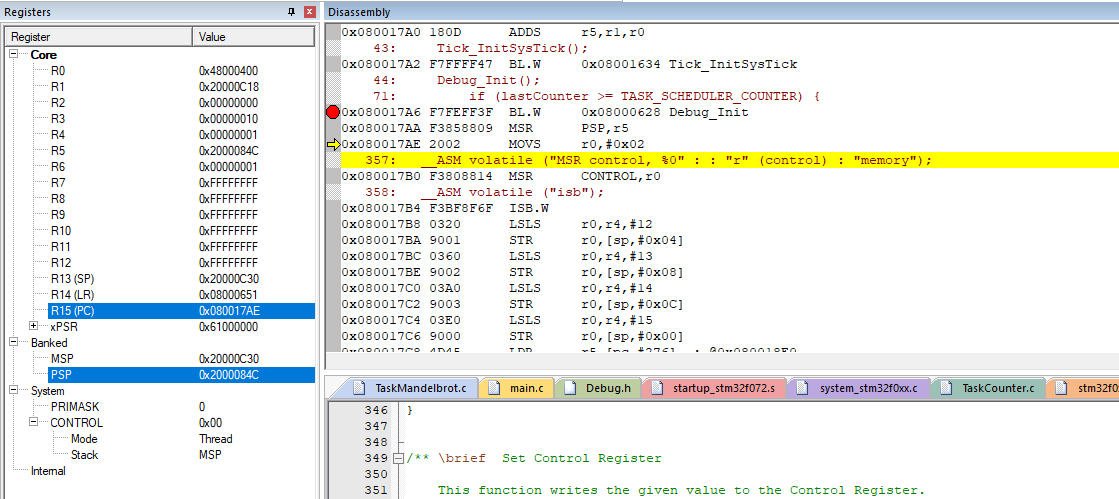
\includegraphics[width=\textwidth]{Images/psp_init.png}

Schließlich der Switch von MSP auf PSP durch einen Pipeline-Flush und dadurch das laden von Instruktionen vom PSP:
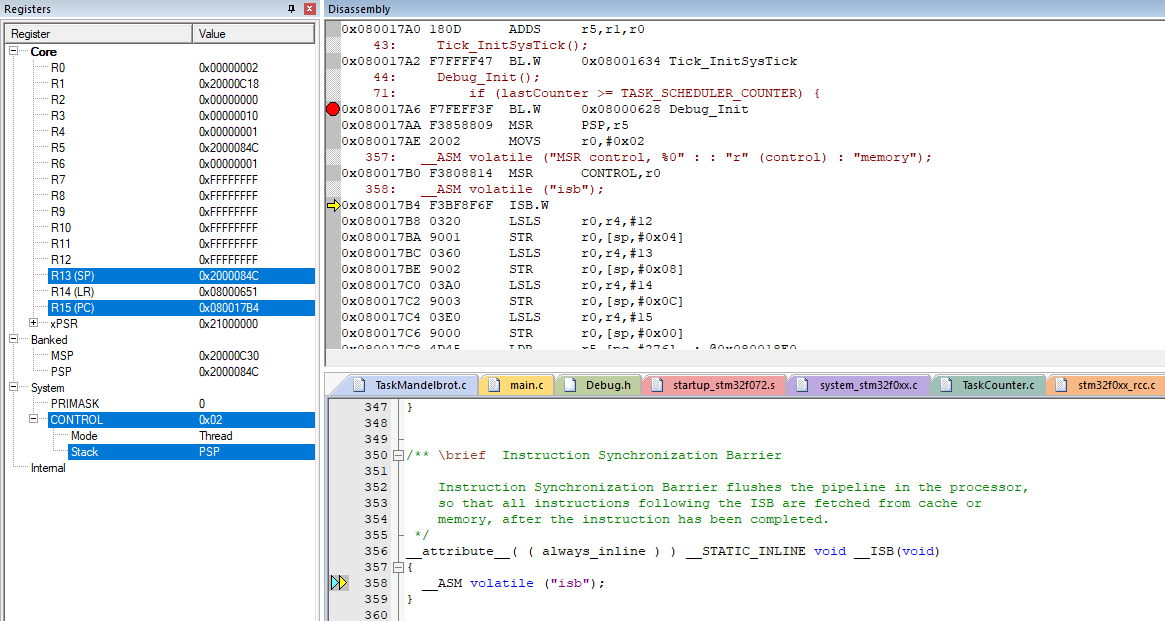
\includegraphics[width=\textwidth]{Images/psp_switch.png}

Somit läuft der Code der Superloop mit all ihren Tasks immer auf dem PSP. 
Auf den MSP muss jedoch nicht gewechselt werden.
Da die ISRs immer auf dem Master-Stack arbeiten erforlgen die Stack-Switches hier automatisch:
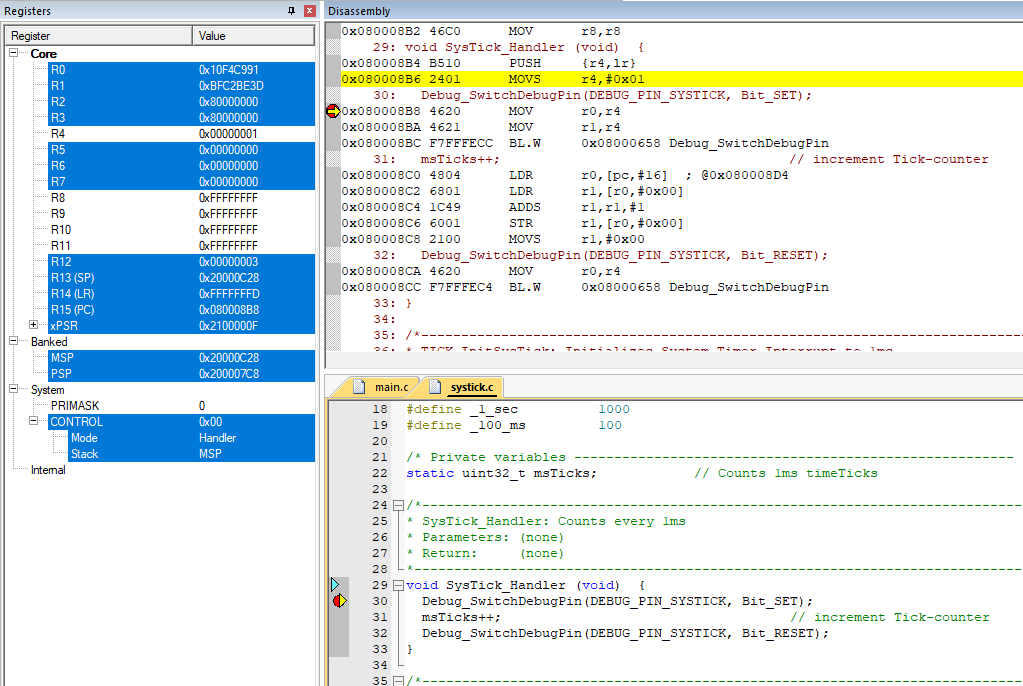
\includegraphics[width=\textwidth]{Images/isr.png}

%\clearpage

%\section{Quellcode}

% \subsection{UE1\_DLL.h}
% \lstinputlisting{./../../UE1_DLL/UE1_DLL.h}
% 
% \subsection{UE1\_DLL.cpp}
% \lstinputlisting{./../../UE1_DLL/UE1_DLL.cpp}
% 
% \subsection{dllmain.cpp}
% \lstinputlisting{./../../UE1_DLL/dllmain.cpp}
% 
% \subsection{TestDLL.h}
% \lstinputlisting{./../../UE1_DLL_TEST/TestDLL.h}
% 
% \subsection{TestDLL.cpp}
% \lstinputlisting{./../../UE1_DLL_TEST/TestDLL.cpp}
% 
% \subsection{main.cpp}
% \lstinputlisting{./../../UE1_DLL_TEST/main.cpp}

\end{document}
